% !TeX spellcheck = en_US
\documentclass[a4paper,12pt]{article}

\usepackage{fullpage}
\usepackage{fourier}
\usepackage{amsmath}
\usepackage{color}
\usepackage{graphicx}
\usepackage{titlesec}
\usepackage{hyperref}

\titleformat{\subsection}[hang]{\large\bfseries}{\alph{subsection})\quad}{0pt}{}

\newcommand{\twodo}[1]{\textcolor{red}{\textbf{todo:} #1}}

\title{\textbf{Exercises for Image Processing 1}\\Problem Sheet 2}
\author{Axel Brand\\6145101 \and Nour Elfaramawy\\6517858 \and Konstantin M\"ollers\\6313136 \and Sibel Toprak\\6712316}

\begin{document}
	\maketitle
	
	\section{Photometry and TV Imaging}
	
	\subsection{Photometry}
	 For the steps of a staircase to become 'invisible' or indistinguishable from another, the pixels forming the individual steps of the staircase need to 'blend/melt' into each other: there is a very low contrast between color/ brightness levels, forming a homogeneous mass. Several components are affecting individual pixel brightness in images and can contribute to this effect:
	 
	\begin{description}
		\item[Illumination (Spectral Energy):] Very high illumination could lead to the scene not having intense shadows, which makes steps not as distinguishable (this depends on the geometry of the light source and the angle at which the light shines on the stairs). Very low illumination makes color values harder to distinguish in many scenarios (low spectral intensity) and also has an effect on many sensors.
		
		\item[Object Surface Properties:] Object surfaces have an extreme impact on their recognizability. A very smooth or homogeneous texture can contribute to the step not being distinguishable. It can also influence whether the light that hits the surface is rather \emph{absorbed, reflected or scattered}. This, in turn, has an effect on the distinction of shadows thrown by the object.
		
				\begin{figure}[h!]	
					\centering
					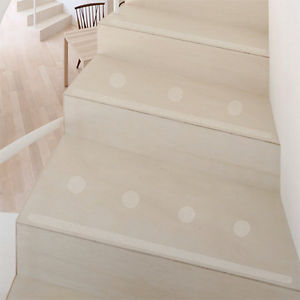
\includegraphics[scale=0.5]{homogene_treppe.JPG}
					\caption{Homogeneous staircase}
				\end{figure}
				
		\item[Sensor Properties:] Different sensors have varying color sensitivity properties (CCD vs CMOS) and are also more or less affected by illumination.
		
		\item[Geometry of the Light Source:] This can contribute to the object not throwing many shadows on certain angles light direction. A very smooth distribution of light will boost surface properties causing the described effect.
		
		\item[Transparency of the Irradiated Medium:] Dust, smoke etc. will influence the amount of light that hits the object's surface and also the amount of reflected light that finally arrives at the sensors.
	\end{description}
	
%TODO: When searching about photometric laws BRDF (Bi-directional Reflectance Distribution Function) is always named, anybody understanding it well enough to say something about the way it contributes here?
% Sibel: Me not really. 
		
	\subsection{TV Images}
	We know that 25 full frames (50 half frames) are shown per second in the PAL standard and that 1 full frame consists of 625 rows\footnote{see last slide of Lecture 3, Image Understanding and Image Formation}. Hence, we can compute the time it takes for one row like so:
	\begin{align*}
		\frac{1 s}{25 \cdot 625} = 0.000064 s = 64\mu s
	\end{align*}
	
	We also know that 1 meter in the real world translates to 10 pixels in the TV image\footnote{See ``The camera optics depict a car of 5m length in 50 pixels'' in the task description}. Based on that, we can convert the velocity of the car moving parallel to the image plane given in $\frac{km}{h}$ into $\frac{px}{\mu s}$:
	\begin{align*}
		50 \frac{km}{h} = 50,000 \frac{m}{h} \Rightarrow 500,000 \frac{px}{h} = \frac{5}{3.6 \cdot 10^{4}} \frac{px}{\mu s} = 0.00013\overline{8} \frac{px}{\mu s}
	\end{align*}
	
	The number of lines lying between the lines 200 and 201 is equivalent to half a visible frame, because the uneven numbered lines starting at line 201 ($201, 203, 205, \dots, 575$) are recorded before the even numbered ones until line 200 ($2, 4, 6, \dots, 200$) in interlaced mode. Knowing that the visible frame comprises 576 rows, the lapse of time between recording the lines 200 and 201 and would be:
	\begin{align*}
	\frac{576}{2} \cdot 64\mu s = 288 \cdot 64\mu s = 18,432 \mu s
	\end{align*}
	
	Now, to compute the offset in pixels between the front end of the car in line 200 and in line 201, we multiply this lapse of time with the velocity previously converted into $\frac{px}{\mu s}$, resulting in an offset of about 3 pixels:
	
	\begin{align*}
	\mathit{offset} = 0.00013\overline{8} \frac{px}{\mu s} \cdot 18,432 \mu s = 2.56 px.
	\end{align*}
	
	In the attached \texttt{E02.py} you can also find a Python implementation.
	
	\section{Color Perception}
	
	\subsection{Image Generation}
	
	We use a \href{https://en.wikipedia.org/wiki/Mandelbrot_set}{Mandelbrot set algorithm} to generate a fractal image. Our implementation is 25 times zoomed into the fractal, shifted about 0.73 units to the right and 0.21 units to the top. The resulting image is shown in figure~\ref{fig:b1}.
	
	\begin{figure}[h!]	
		\centering
		\includegraphics[width=.95\textwidth]{B1.png}
		\caption{\label{fig:b1}B1, the generated image.}
	\end{figure}
	
	Figure~\ref{fig:b1bright} displays the brightness values of B1. The brightness is calculated by the formula taken from the script: $\mathit{brightness} = \frac{R + G + B}{3}$
	
	\begin{figure}[h!]	
		\centering
		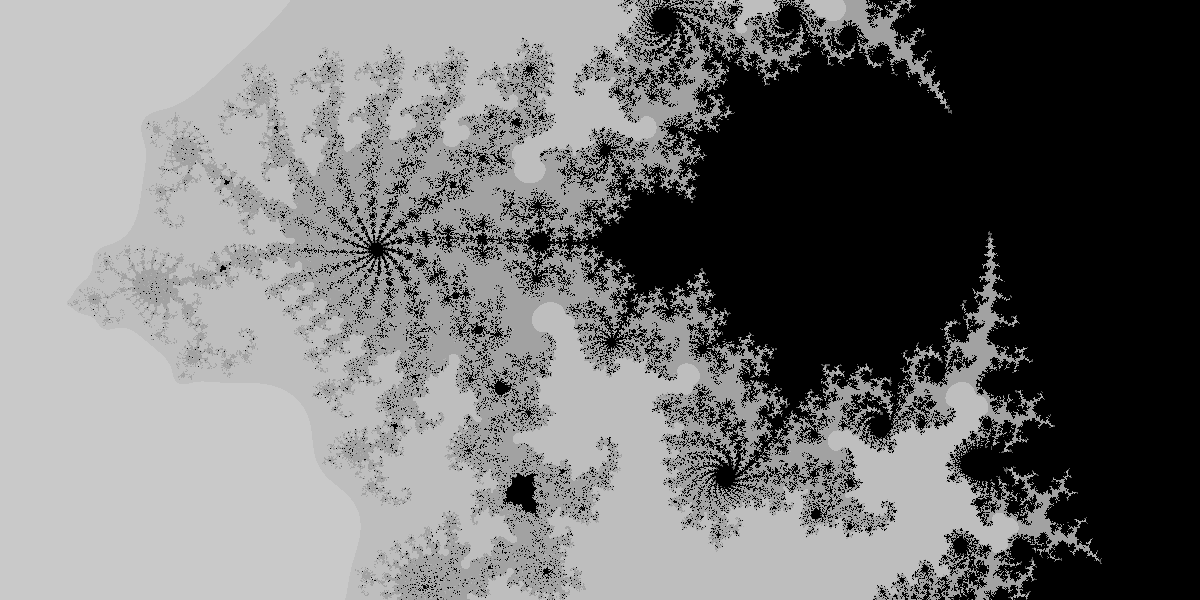
\includegraphics[width=.95\textwidth]{B1_Brightness.png}
		\caption{\label{fig:b1bright}Brightness values of B1.}
	\end{figure}
	
	\subsection{Image Calibration}
	
	The calibrated image is calculated by translating the RGB color model used by \texttt{numpy} to the HLS color model, which can be achieved by the \texttt{colorsys} library. In the HLS model, we fix the lightness to a value of 0.5, translate the resulting color back to RGB, and set the triple back on the image plane. The resulting image is in figure~\ref{fig:b2}.
	
	\begin{figure}[h!]	
		\centering
		
\includegraphics[width=.95\textwidth]{B2.png}
		\caption{\label{fig:b2}B2, the calibrated image.}
	\end{figure}
	
	As you can see in figure~\ref{fig:b2bright}, all brightness values are now the same.
	
	\begin{figure}[h!]	
		\centering
		
\includegraphics[width=.95\textwidth]{B2_Brightness.png}
		\caption{\label{fig:b2bright}Brightness values of B2.}
	\end{figure}
\end{document}